\documentclass[a4paper,11pt]{article}
\usepackage{a4wide}
\usepackage[english]{babel}
\usepackage{url}
\usepackage[latin1]{inputenc}
%\usepackage[small,bf,hang]{caption2}
\usepackage{xspace}
\usepackage{graphicx}
\usepackage{listings}
\usepackage{color}  
\usepackage[toc,page]{appendix}
\usepackage{subcaption}
\usepackage{pdflscape}
\usepackage{fixltx2e}

\newcommand{\HRule}{\rule{\linewidth}{0.5mm}}
\definecolor{mygreen}{rgb}{0,0.6,0}
\definecolor{mygray}{rgb}{0.5,0.5,0.5}
\definecolor{mymauve}{rgb}{0.8,0.4,0.2}
\definecolor{dkgreen}{rgb}{0,.6,0}
\definecolor{dkblue}{rgb}{0,0,.6}
\definecolor{dkyellow}{cmyk}{0,0,.8,.3}
\definecolor{gray}{gray}{0.6}

\lstset{
  backgroundcolor=\color{white},   % choose the background color; you must add \usepackage{color} or \usepackage{xcolor}
  basicstyle=\footnotesize,        % the size of the fonts that are used for the code
  breakatwhitespace=false,         % sets if automatic breaks should only happen at whitespace
  breaklines=true,                 % sets automatic line breaking
  captionpos=b,                    % sets the caption-position to bottom
  commentstyle=\color{mygreen},    % comment style
  deletekeywords={...},            % if you want to delete keywords from the given language
  escapeinside={\%*}{*)},          % if you want to add LaTeX within your code
  extendedchars=true,              % lets you use non-ASCII characters; for 8-bits encodings only, does not work with UTF-8
  frame=single,                    % adds a frame around the code
  keepspaces=true,                 % keeps spaces in text, useful for keeping indentation of code (possibly needs columns=flexible)
  keywordstyle=\color{blue},       % keyword style
  language=C++,                 % the language of the code
  morekeywords={*,...},            % if you want to add more keywords to the set
  numbers=none,                    % where to put the line-numbers; possible values are (none, left, right)
  numbersep=5pt,                   % how far the line-numbers are from the code
  numberstyle=\tiny\color{mygray}, % the style that is used for the line-numbers
  rulecolor=\color{black},         % if not set, the frame-color may be changed on line-breaks within not-black text (e.g. comments (green here))
  showspaces=false,                % show spaces everywhere adding particular underscores; it overrides 'showstringspaces'
  showstringspaces=false,          % underline spaces within strings only
  showtabs=false,                  % show tabs within strings adding particular underscores
  stepnumber=2,                    % the step between two line-numbers. If it's 1, each line will be numbered
  stringstyle=\color{mymauve},     % string literal style
  tabsize=2,                       % sets default tabsize to 2 spaces
  title=\lstname                   % show the filename of files included with \lstinputlisting; also try caption instead of title
}

\setlength{\parindent}{0cm}             % Inspringen van eerste lijn van paragrafen is niet gewenst.
\graphicspath{{figs/}}               % De plaars waar latex zijn figuren gaat halen.
\newcommand{\npar}{\par \vspace{2.3ex plus 0.3ex minus 0.3ex}}

\begin{document}

\begin{titlepage}
\pagenumbering{gobble}
\begin{center}

% Upper part of the page. The '~' is needed because \\
% only works if a paragraph has started.

\includegraphics[width=0.4\textwidth]{./logo}~\\[1cm]

% Title
\HRule \\[0.4cm]
\huge \textbf{Design of Multimedia Applications}
\HRule \\[0.4cm]
{ \huge \bfseries Report 1: Error Concealment \\[0.4cm] }
\HRule \\[0.4cm]

% Author and supervisor
\begin{minipage}{0.4\textwidth}
\begin{flushleft} \large
\emph{By:}\\
Andrea \textsc{Accogli}\\
Michiel \textsc{Creve}\\
Andreas \textsc{De Lille}\\
\end{flushleft}
\end{minipage}

\vfill

% Bottom of the page
{\large \today}

\end{center}
\end{titlepage}

\tableofcontents
%\listoffigures
%\listoftables

\newpage
\pagenumbering{arabic}
\setcounter{page}{1}
\section[Pseudocode and explanatory notes for the methods that have been implemented in
Exercises 2.B, 2.C, 3.B, 3.C, and 3D, paying particular attention to the way edge
information and content-adaptivity were leveraged.]{}\label{Q1}

\subsection{2.B}
In order to reduce the interpolation complexity, a similar technique as 2.A is applied. First the function f has been modified so that only two macroblocks are used for the interpolation (the two closest in case more than two macroblocks are available). Secondly, the function f originally performed the interpolation if there was at least one valid neighboring macroblock. New pixels values would be overridden if the macroblock has more neighbours. In other words, the method would perform the interpolation multiple times. This behaviour is removed. This is done by adding a new input parameter ($neighbs$) to f, which specifies the number of surrounding macroblocks required to enable the interpolation. The control block will only interpolate if the number of surrounding macroblocks is bigger than "neighbs" (and not bigger than zero, as before). In the following pseudocode, the changes in respect to the first version of f will be highlighted.
\vspace{1em}
\begin{lstlisting}[frame=single]
void f(Macroblock, exist_l/r/t/b, MBstate, MBx, neighbs, frame){
	   ...
	// No changes in respect to the original f
     ...
	// New "if" block to check the number of surrounding macroblocks:
	if exist_l + exist_r + exist_t + exist_b > neighbs{
		for (int i = 0; i < 16; ++i)	{
			for (int j = 0; j < 16; ++j){
				if (neighbs > 1 and more than two neighbours are available){
                	if top is closest: set exist_bottom to false and vice versa
                    if right is closest: set exist_left to false and vice versa
		...
      //Pixel interpolation
}
\end{lstlisting}

\subsection{2.C}
The body of the $conceal\_spatial\_2$ method is the same as the 2.B exercise. The difference between $conceal\_spatial\_2$ and $conceal\_spatial\_3$ is the function that is used for the error concealment. For $conceal\_spatial\_3$, f2 is used instead of f. Only f2 is discussed here.

\vspace{1em}
\begin{lstlisting}[frame=single]

void f2(Macroblock, exist_l/r/t/b, State, Macroblock_index, frame){
	
	declare both horizontal and vertical 3x3 Sobel kernel

	// Determine which borders of the missing macroblock are present

	for(border = upper, right, lower, left)
		if border macroblock exists
			assign left border to macroblock object 
		else set exist_border to zero

	// Extract edge data from existing borders and calculate gradients and slopes
	for(border = upper, right, lower, left)
		if border exists
			determine x_gradient of border by convolving Sobel kernel with MB edge
			determine y_gradient of border by convolving Sobel kernel with MB edge
			// Note that we leave 1 rown/column open between the missing MB, and
			// The center of the convolution (we convolve with row/column 1 or 14
			// instead of 0 or 15). Otherwise, we would need pixels from the missing
			// MB. For the same reason, we only use 14 pixels per edge (instead of 
			// 16). When using 16, we would also need pixels of the upper-right, 
			// lower-right, ... macroblock (8-connected instead of 4-connected).
			
			gradient = sqrt(x_gradient^2 + y_gradient^2)
			slope = 1.0/tan(y_gradient / x_gradient)			

	// Determine dominant gradient direction
	calculate mean of all gradients
	calculate variance of all gradients (= sum(gradient-mean)/sizeof(gradients))
	
	/////// dominant direction = weighing the slopes with their gradient
	/////// = sum(gradient*slope) / sum(gradient)
	for all gradients
		if gradient > variance
			numerator = abs(gradient)*slope
			denominator = abs(gradient)

	dominant direction = numerator / denominator

	// Interpolate the pixels in dominant direction 
	
  for(all pixels in macroblock)
		////// First: luma values (16x16)
		slope = 1/tan(dominant direction)
	
		////// Per pixel we want to conceal, we need 2 border pixels which we will
		////// to find the concealed pixel value.
		////// P1:
		if slope > 0			//P1 will be part of left or upper border
			find border pixel with the dominant slope
			if needed border macroblock exists
				assign border pixel luma value to p1
			else if other border macroblock exists (left <-> upper)
				assign closest luma value to p1 (will be left[0][15] or upper[15][0])
			else
				perform spatial interpolation, described in conceal_spatial_2
		else					//P1 will be part of the left or lower border
					find border pixel with the dominant slope
			if needed border macroblock exists
				assign border pixel luma value to p1
			else if other border macroblock exists (left <-> lower)
				assign closest luma value to p1 (will be lower[0][0] or left[15][15])
			else
				perform spatial interpolation, described in conceal_spatial_2
	
		////// P2:
		if slope > 0			//P2 will be part of upper or right border
			repeat the above steps
		else					// P2 will be part of right or lower border
			repeat the above steps
	
		calculate distances from pixel to p1 and p2
	
		// Now we interpolate the pixel luma values, weighted with the distances
		concealed pixel luma = 1/(dist1 + dist2)*(dist2*p1_luma + dist1*p2_luma)	
	}
	////// Second: cb and cr values (8x8)    
	do exactly the same as above, but for 8x8 instead of 16x16		
}

\end{lstlisting}

\subsection{3.B}
This method will first divide the macroblock (of size 16x16) into smaller subblocks of a fixed size (2,4,8 or 16). Then a motion vector is calculated for each subblock. Complex reduction is used. At first the average luma value of each subblock is calculated and then searched within a window around the macroblock. This proved to be too slow for the results. To make this method faster, the calculation changed to interpolation of the motion vectors of the surrounding macroblocks. This is done in the same way as 2B, but now for both the x and y component of the motion vector. If the given frame is a P frame or a predictively coded frame, then spatial interpolation is used instead. 

\begin{lstlisting}[frame=single]
if (p_frame): use spatial
else
	foreach macroblock mb
    	if (mb->isMissing)
        	interpolate motion vector
            fill the frame
            if (error of block > 25) 
            	put in queue
	foreach element in queue: conceal_spatial
\end{lstlisting}

\subsection{3.C}
This method is a newer, extended version of 3B, where extra code is added to tackle the complex pattern.
This method uses auto-selection of the subblock sizes. All the possible sizes are tested and the best one is used.
This works great if the frames 'overlap', so that we can reconstruct one frame by using previous frames. However when the next frame is completly different, then the previous frame 'shines through' the new frame. This is certainly the case with the complex pattern. Therefore the error is calculated by checking which part of the edges match. If this error gets too big then spatial interpolation is used instead.
\npar
This spatial interpolation is done in descending neighbour order. The idea is that more available neighbours lead to better concealments. To do this elegantly, a priority queue is used. Changing priorities in this queue proved to be less efficient. To solve this all neighbours of each concealed macroblock are added to the queue. If the macroblock has more neighbours then his predecessor then he will come out first. A downside of this is that we have to clean the queue after each iteration.
\vspace{1em}
\begin{lstlisting}[frame=single]
if (p_frame): use spatial
else
	foreach macroblock mb
    	if (mb->isMissing)
        	for each subsize
        		interpolate motion vector
            	fill the frame
            	calculate the error
                
			copy the values of the best result into the macroblock
                
            if (best_error > 25): put in priority queue
            
	foreach element in queue
    	conceal_spatial
        put neighbours in priority queue
        clean the priority queue
\end{lstlisting}

\subsection{3.D}
This method is similar to 3C, but uses dynamic blocksizes. This means that one macroblock can be covered by subblocks of different sizes. The method starts by concealing the whole macroblock. Then it goes over the different sizes (8,4,2) and checks whether or not the error has decreased. Only when the error decreases, the new values are kept.

\vspace{1em}
\begin{lstlisting}[frame=single]
if (p_frame): use spatial
else
	foreach macroblock mb
    	if (mb->isMissing)
        	Do a motion concealment with subsize = 16, so the whole block is concealed.
            
        	for each subsize
            	for each subblock
                	create temp macroblock
                	conceal the subblock (of the temp macroblock)
                    if err < best_err
                    	swap the pixel values in the macroblock with the ones from the temp block
                
            if (best_error > 25): put in priority queue
                
	foreach element in queue
    	conceal_spatial
        put neighbours in priority queue
        clean the priority queue
\end{lstlisting}
\section[The rationale of why these methods were chosen, and a discussion of their advantages and disadvantages.]{}

\subsection{Spatial interpolation}
Spatial interpolation techniques have many pros: since they only work just on the current frame, retransmission or knowledge about previous frames isn't required. They are also very simple to implement and yield satisfactory results. Even though it's a good compromise, details are often concealed by unnatural blurry areas that can easily be seen by the human eye. An improvement to this method is to combine it with motion estimation. However, spatial interpolation is fundamental when the frame changes completely, because concealing errors using previous frames would then lead to wrong results: the previous frame will still be partially visible.

\subsection{Edge detection}
This method is based on the paper 'Flexible Error Concealment for H.264 Based on Directional Interpolation' by O. Nemethove, A. Al-Moghrabi and M. Rupp, in which the described methods seemed to yield good results. The authors propose both a solution with one dominant direction and an extended version which divides a macroblock in sections. The method implemented in this assignment is the simpler method with one dominant direction.
\npar
The method works well when there are not too many blocks missing (the simple error pattern). If sufficient edge data is available, the method usually finds a correct dominant direction. However, if a lot of the neighbours are missing (the complex error pattern), the dominant direction won't always be correct. This results in edges that are uncorrectly being prolonged. This explains why the result when applying the complex error pattern is not optimal, while the result when applying the simple error pattern is acceptable. In case of the simple pattern, the method only makes observable mistakes at the edges of e.g. persons, but the video stays 'watchable' at any time.
\npar
Another (minor) drawback of this method is that sometimes there are two (or more) dominant edges which should have been prolonged (= paritioning the macroblock in segments). In these cases the edges will be less efficient. 
\npar
As an example, a screenshot of a concealed frame is provided in Figure \ref{fig:2C} in Appendix \ref{app:Q2}. Figure \ref{fig:2C_prior} shows the frame prior to this concealed frame. Block 1 shows a wrongly prolonged edge. The arm of the person is 'smudged out' into the background. Block 2 illustrates a case where a missing macroblock is concealed correctly, so that a viewer can barely notice that this block was missing and has been concealed. The nose of the person in block 3 more or less has a correct edge direction. Though, in this case the color values don't match the values of the original frame.\\
Please note that there are many more concealed macroblocks present in the frame, while as a viewer you can only notice a few of them.
\clearpage
\subsection{Motion estimation}
Motion estimation works excellent when the new frame overlaps with the previous frame. If the camera moves slow then the no motion estimation already works pretty good. Also the provided method which uses the best fitting motion vector of the surrounding neighbours yields good results. The lab exercise was to improve this method by first using smaller subblocks with fixed sizes, then auto selecting the best size and finally creating a dynamic system. The output will be surprisingly similar, as explained in Q5.
\section[The results of all quality and time measurements (provide information about the
PC configuration used in order to put the time measurements in context).]{}

\subsection{Timings explained}
Both the simple and complex error pattern are used for the beowulf sequence.
The conceal time is calculated by timing each frame, the sum of these times is then divided by the amount of missing frames. Note that we calculate the average time it takes to conceal a frame, not the time it takes to load a frame.

\subsection{Setup}
PC Configuration used for the measurements: an Intel i5, 2 cores, 4 threads @2.5ghz with 8GB dual-channel DDR3 @798Mhz RAM. The GPU is an Integrated Intel Hd graphics 4600 + NVIDIA GeForce GT 740M (2048MB dedicated RAM). The HD is a 700GB SATA-III 5400 RPM.

\subsection{Results}
A comprehensive table with the timings, PSNR and SSIM values is included in appendix \ref{Q3:timings}. The results will be further explained in question 4.
\section[A comparison of the different results, as well as an explanation of the relation
between the results.]{}
As you can see in Appendix \ref{app:Q4}, explaining the results is more or less straight forward. One can see that the spatial methods (2A and 2B) and the zero motion method (3A) are all very fast for the simple pattern, due to their simplicity. 3B takes somewhat more processing, how much more depends on the size of the subblocks. The edge detection (2C) is somewhat slower than 3B, but still uses reasonable time. 3C and 3D are both very complex, even after reductions and are therefore much slower. 
\npar
The complex pattern has some differences, firstly the motion methods slowed down by a constant factor. This is normal, since more macroblocks have to be concealed. The story for the spatial methods is different, 2B is relatively much more slower than 3B, this is due to the fact that 2B keeps looking for the blocks with the most neighbours, which causes overhead. 2C uses the same body as 2B, only the interpolation method (f $\rightarrow$ f2) is different. This declares why 2C is also very slow.
\section[Evaluate the performance of the different sub-macroblock sizes for error conceal-
ment and compare this with the results for an adaptive sub-macroblock conceal-
ment method (Exercise 3.D). Perform an evaluation of the objective and subjective
quality.]{}

If the smaller subblocks are used, the processing time increases. However, as you can see in Appendix \ref{Q3:timings} the PSNR and SSIM values do not differ that much. This seems strange, but can be explained as follows: the motion in the frame tends to be consistent over the whole frame. If the camera moves, then the whole frames moves, this consistency causes the motion vectors mv\textsubscript{b}, mv\textsubscript{c}, mv\textsubscript{d} and mv\textsubscript{e} of Figure \ref{Q5:motions} in Appendix \ref{Q5} to be (almost) equal. Therefore the interpolation doesn't have a lot of impact. This impact would be more visible when there is a new shot, but our methods will detect the huge error and correct it by switching to spatial interpolation. This also explains why 3C and 3D have similar SSIM and PSNR values, but are slower due to the fact that they do more work.
\section[Conclusions regarding the comparison of the different results (for the spatial and
temporal techniques separately, as well as for the comparison of both approaches).]{}
The spatial methods are fast for the simple pattern, but become a lot slower for the complex pattern. This is due to the overhead it takes to search the blocks with most neighbours. This does not occur for the motion methods. These methods are optimized for speed. They use motion on all blocks, and store the blocks that have too big errors in a priority queue. These blocks are handled in order of present neighbours. Thus, here the overhead is reduced by using a priority queue.
\section[An answer, with explanation, to the following questions:]{}
\subsection[Can a clear winner be found among all techniques and groups of techniques? If so, what would be a possible reason for not choosing the best candidate
(thus, choosing another technique)? If not, which factors decide which technique is best?]{}
\subsection[When you do a visual inspection of the reconstructed sequences, do you get
the same results? If so, what conclusions can be drawn from this experiment? If not, what are the main differences and what can be concluded?]{}

It is not possible to select a clear winner, because the output heavily depends on the given frame. For instance if the frame has colors that melt together, then the spatial interpolation would give good results. Spatial interpolation is not good at concealing edges, because the result is usually blurry. If a static text is shown in front of a moving background, then the text will be easier to read with zero motion concealment, this is visible in Figure \ref{Q7:zerotwee} of Appendix \ref{Q7}. 
\npar
Edge detection works good when there are sufficient edges. Too much different edges and it becomes confused, too few and the edge detection will have to fall back on spatial interpolation. The neighbours also have influence: if the missing macroblock has a lot of neighbours, then the edge detection will succeed in finding and restoring the edge. However if a lot of the neighbours are missing, then the edge method will have a hard time finding the edge. 
\npar
Generally the spatial methods give better SSIM values for the simple pattern whereas the motion methods are better to tackle the complex pattern, this is shown in Appendix \ref{app:Q10} and is also visible in the output, see Figure \ref{Q7:edgemotion} and Figure \ref{Q7:edgemotioncomplex} in Appendix \ref{Q7}.


\section[What would be the advantages and disadvantages of client-side buffering?]{}

Client side buffering can hide most network problems. A sudden drop in network speed could be hidden easily by using frames out of the buffer while waiting for the network to catch up. When the buffer is large enough, then it's even possible to retransmit lost macroblocks. However the retransmission needs to happen within a short time window. The request for retransmission and retransmission itself has to be completed before the frame is needed. Even then there is no guarantee that no macroblocks will get lost. Note that buffering also requires more resources and is not always possible (e.g. livestreaming).
\section[Given the complex error pattern, what is the highest PSNR value obtained for the
entire Beowulf video sequence (calculated as the average of all frame PSNR values),
for Exercise 2.B, Exercise 2.C, Exercise 3.C, and Exercise 3.D? Plot the different
PSNR values in a summarizing table.]{}
The highest average PSNR value obtained is that of exercice 3.C: 35.470105 dB. A summarizing table for exercice 2.B, 2.C, 3.C and 3.D is plotted below:

\begin{table}[h]
\centering
\begin{tabular}{l|l|l|l|l|}
\cline{2-5}
                                            & \multicolumn{1}{c|}{\textbf{2.B}} & \multicolumn{1}{c|}{\textbf{2.C}} & \multicolumn{1}{c|}{\textbf{3.C}} & \multicolumn{1}{c|}{\textbf{3.D}} \\ \hline
\multicolumn{1}{|l|}{\textbf{Average PSNR}} & 32.668692 dB                         & 32.113921 dB                         & 35.470105 dB                        & 35.367707 dB                        \\ \hline
\end{tabular}
\end{table}
\section[Is there a clear correlation between the PSNR and SSIM; and does the SSIM better match the perceived quality.]{}
PSNR (Peak signal-to-noise ratio) is known for its inconsistency with human eye perception. The idea behind PSNR is that a noise signal is added to the original signal. It doesn't take into account things where humans are sensitive to (e.g. the structure in an image).
SSIM (Structural Similarity) however does take the human eye perception into account. To find the structural similarity of two images, it takes into account the luminance, contrast and structure (to which a human is sensitive).
\npar
In short: PSNR is based upon perceived errors in an image, while SSIM is based upon perceived change in structural information between 2 images. Thus, there is no clear correlation between the PSNR values and SSIM values. This can also be seen when comparing the graphs in Appendices \ref{app:Q9} and \ref{app:Q10}: when we look to the results with the simple pattern, exercise 3 (motion) seems to be the best regarding to the PSNR values (highest values). On the contrary, when we look to the SSIM values, exercise 2 (spatial) seems to yield the best results.
\section[Give a description of the complexity reduction techniques you have introduced in Exercise 3.D. How did the result of the algorithm match with the expected behavior?
Can you describe other algorithms you did not implement?]{}
The original assignment was to create the block sizes dynamically. As mentioned earlier, the searching of luma values to determine the motion vectors turned out to be too slow. To solve this, interpolation of the surrounding motion vectors is used. This resulted in a huge performance gain.
\npar
To reduce the computation time, two macroblocks are used. The previous one holds the macroblock that has been optimized so far. The new one holds the result of the new iteration. For example: one block of 8x8 in the previous one could be replaced by 4 blocks with size 4x4 in the new block. Once that new block is formed, the error is calculated. If this error is lower then the error of the previous one, the blocks are swapped, else the new block is discarded. 

\newpage
\begin{appendices}

\section{Q2}\label{app:Q2}

\subsection{2C}

\begin{figure}[!h]
  \centering
  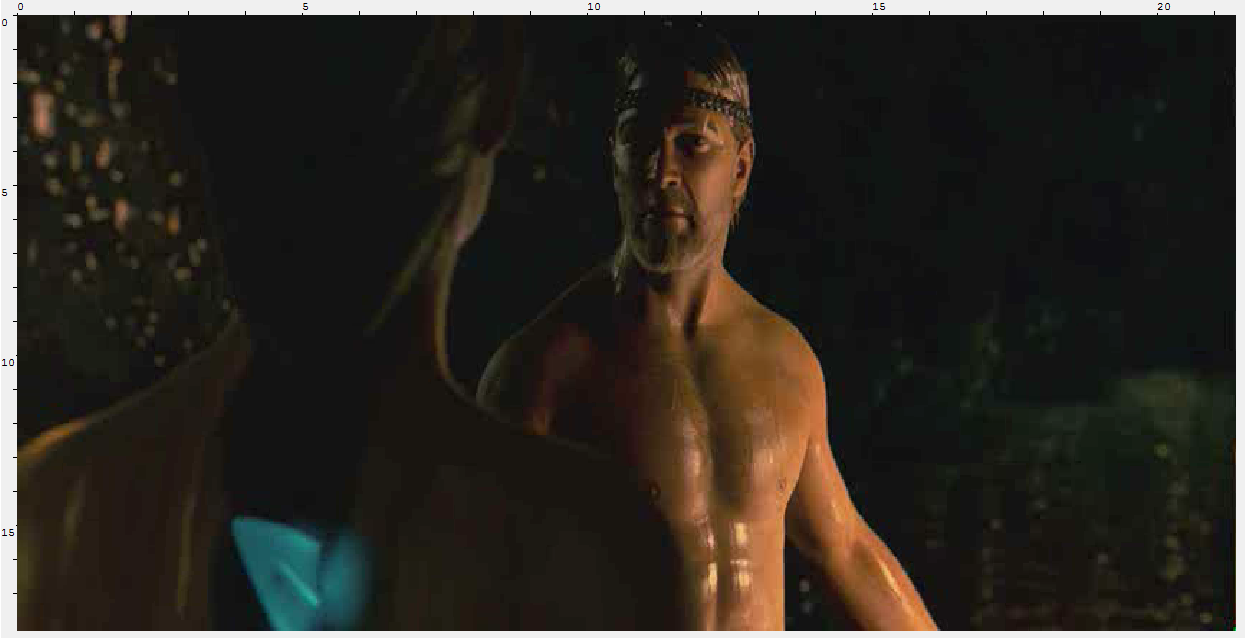
\includegraphics[width=\textwidth]{2C_mistakes_prior}
  \caption{Frame prior to concealed frame taken from the solution to exercice 2C (edge detection).} 
  \label{fig:2C_prior}
\end{figure}

\begin{figure}[!h]
  \centering
  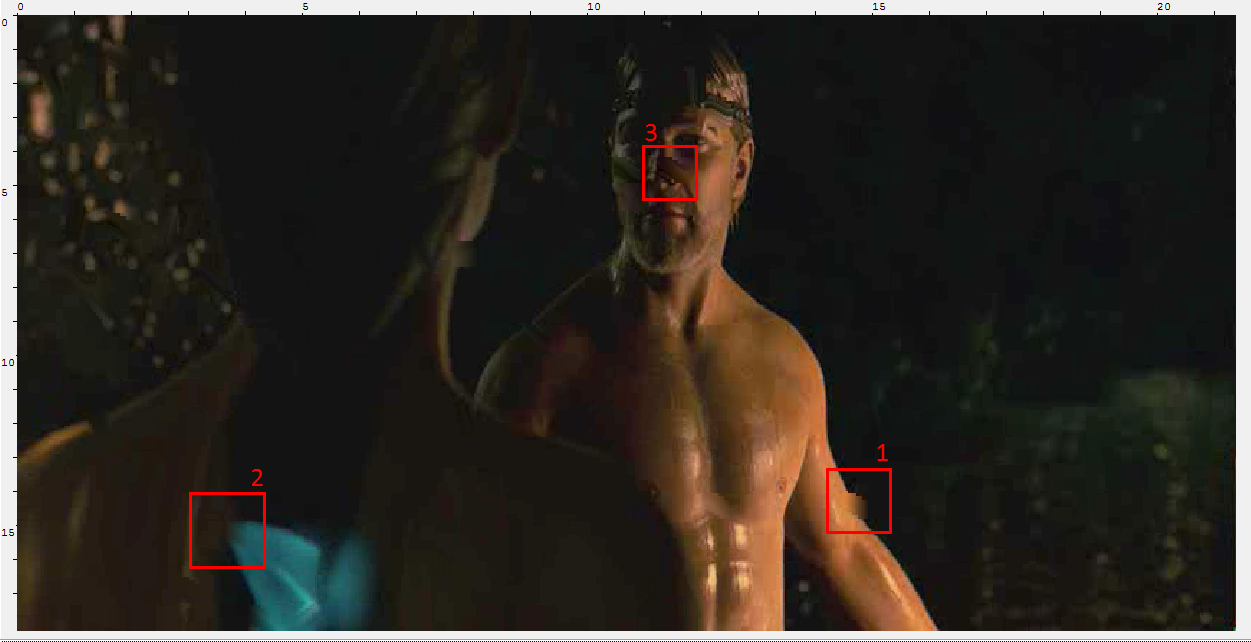
\includegraphics[width=\textwidth]{2C_mistakes}
  \caption{Concealed frame taken from the solution to exercice 2C (edge detection).} 
  \label{fig:2C}
\end{figure}

\newpage

\section{Q3: Timings}\label{Q3:timings}
\begin{table}[h]
\begin{tabular}{|l|l|l|l|l|l|}
\hline
\textbf{Frame}           & \textbf{AVG (s/frame)} & \textbf{total} & \textbf{PSNR} & \textbf{SSIM} & \textbf{AVG (fps)} \\ \hline
\textbf{2A simple}       & 0,000857               & 0,132          & 38,58747      & 0,937994      & 1166,667           \\ \hline
\textbf{2A complex}      & 0,002474               & 0,381          & 22,52592      & 0,520955      & 404,1995           \\ \hline
\textbf{2B simple}       & 0,001299               & 0,2            & 39,74085      & 0,940161      & 770                \\ \hline
\textbf{2B complex}      & 0,299948               & 46,192         & 32,66869      & 0,898557      & 3,333911           \\ \hline
\textbf{2C simple}       & 0,012948               & 1,994          & 39,4913       & 0,938137      & 77,2317            \\ \hline
\textbf{2C complex}      & 10,41379               & 1603,724       & 32,11392      & 0,893201      & 0,096026           \\ \hline
\textbf{3A simple}       & 0,000506               & 0,078          & 39,28378      & 0,927515      & 1974,359           \\ \hline
\textbf{3A complex}      & 0,000844               & 0,13           & 35,46008      & 0,879678      & 1184,615           \\ \hline
\textbf{3B (2) simple}   & 0,010292               & 1,585          & 39,82269      & 0,933798      & 97,16088           \\ \hline
\textbf{3B (2) complex}  & 0,081987               & 12,626         & 35,36771      & 0,896592      & 12,19705           \\ \hline
\textbf{3B (4) simple}   & 0,009351               & 1,44           & 39,82269      & 0,933798      & 106,9444           \\ \hline
\textbf{3B (4) complex}  & 0,073208               & 11,274         & 35,36771      & 0,869592      & 13,65975           \\ \hline
\textbf{3B (8) simple}   & 0,007273               & 1,12           & 39,82269      & 0,933798      & 137,5              \\ \hline
\textbf{3B (8) complex}  & 0,071643               & 11,033         & 35,36771      & 0,896592      & 13,95813           \\ \hline
\textbf{3B (16) simple}  & 0,007156               & 1,102          & 39,82269      & 0,933798      & 139,7459           \\ \hline
\textbf{3B (16) complex} & 0,064987               & 10,008         & 35,36771      & 0,896592      & 15,38769           \\ \hline
\textbf{3C simple}       & 0,031623               & 4,87           & 39,82269      & 0,933798      & 31,62218           \\ \hline
\textbf{3C complex}      & 0,157032               & 24,183         & 35,47011      & 0,892084      & 6,36811            \\ \hline
\textbf{3D simple}       & 0,045922               & 7,072          & 39,82269      & 0,933798      & 21,77602           \\ \hline
\textbf{3D complex}      & 0,240383               & 37,019         & 35,36771      & 0,896592      & 4,160026           \\ \hline
\end{tabular}
\end{table}

\newpage

\section{Q4}\label{app:Q4}

\begin{figure}[!h]\label{fig:time_simple_pattern}
  \centering
  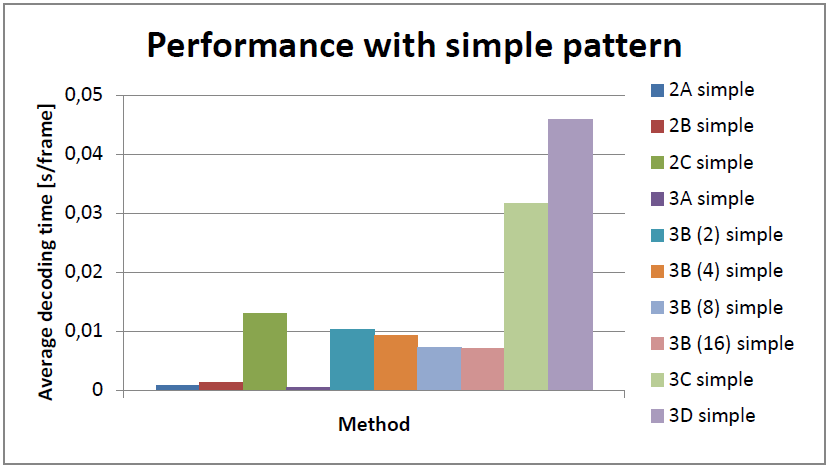
\includegraphics[width=.9\textwidth]{time_simple}
  \caption{Comparison of frame concealment time of all methods with the simple error pattern.} 
\end{figure}

\begin{figure}[!h]\label{fig:time_complex_pattern}
  \centering
  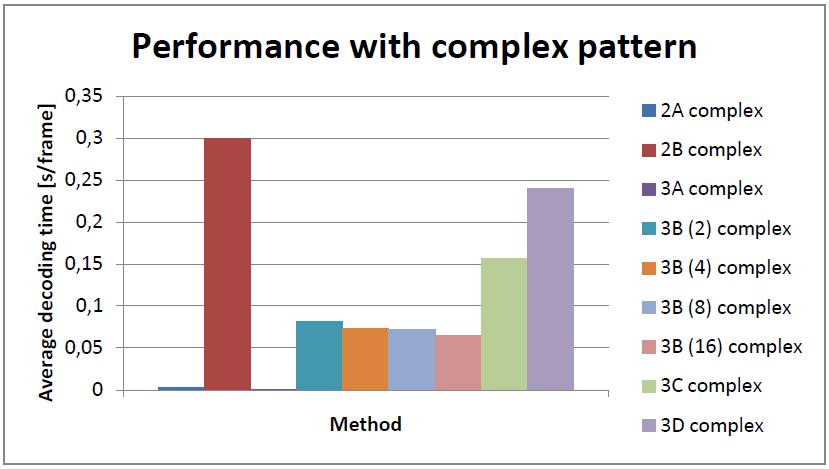
\includegraphics[width=.9\textwidth]{time_complex}
  \caption{Comparison of frame concealment time of all methods with the complex error pattern. The value of 2C has been left out, because it is too high (10,4138). This avoids that graph becomes unreadable.} 
\end{figure}

\newpage

\section{Q5}\label{Q5}
\subsection{Motion vectors}
\begin{figure}[!h]
  \centering
  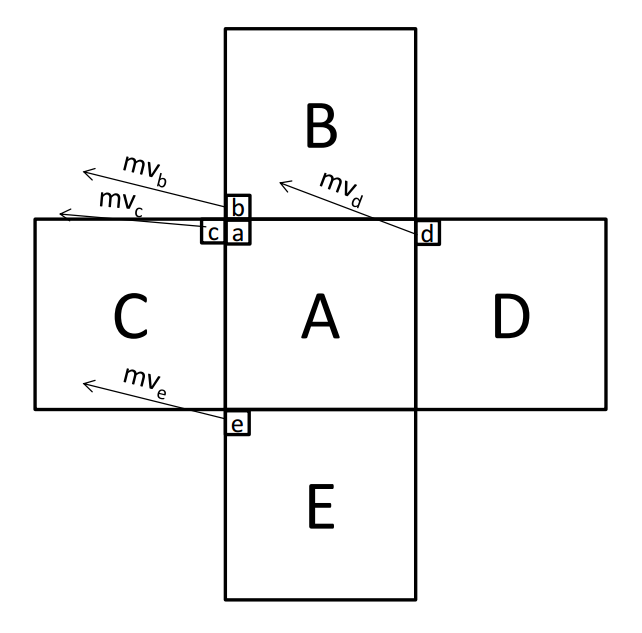
\includegraphics[width=.9\textwidth]{motions}
  \caption{The motions is consistent in the whole frame, therefore the calculated motion vector will be almost the same.} 
  \label{Q5:motions}
\end{figure}

\clearpage

\section{Q7}\label{Q7}
\subsection{Zero motion compared to motion estimation}
\begin{figure}[ht]
\centering
\begin{subfigure}{\textwidth}
  \centering
  
\includegraphics[width=.9\textwidth]{zero}
  \caption{zero motion}
\end{subfigure}\\
\begin{subfigure}{\textwidth}
  \centering
  
\includegraphics[width=.9\textwidth]{tweepertwee}
  \caption{Motion estimation with subblock of size 2}
\end{subfigure}
\caption{Zero motion (3A) compared with non-dynamic motion estimation (3B).}
\label{Q7:zerotwee}
\end{figure}

\clearpage

\subsection{Edges compated to motion estimation - simple pattern}
\begin{figure}[ht]
\centering
\begin{subfigure}{\textwidth}
  \centering
  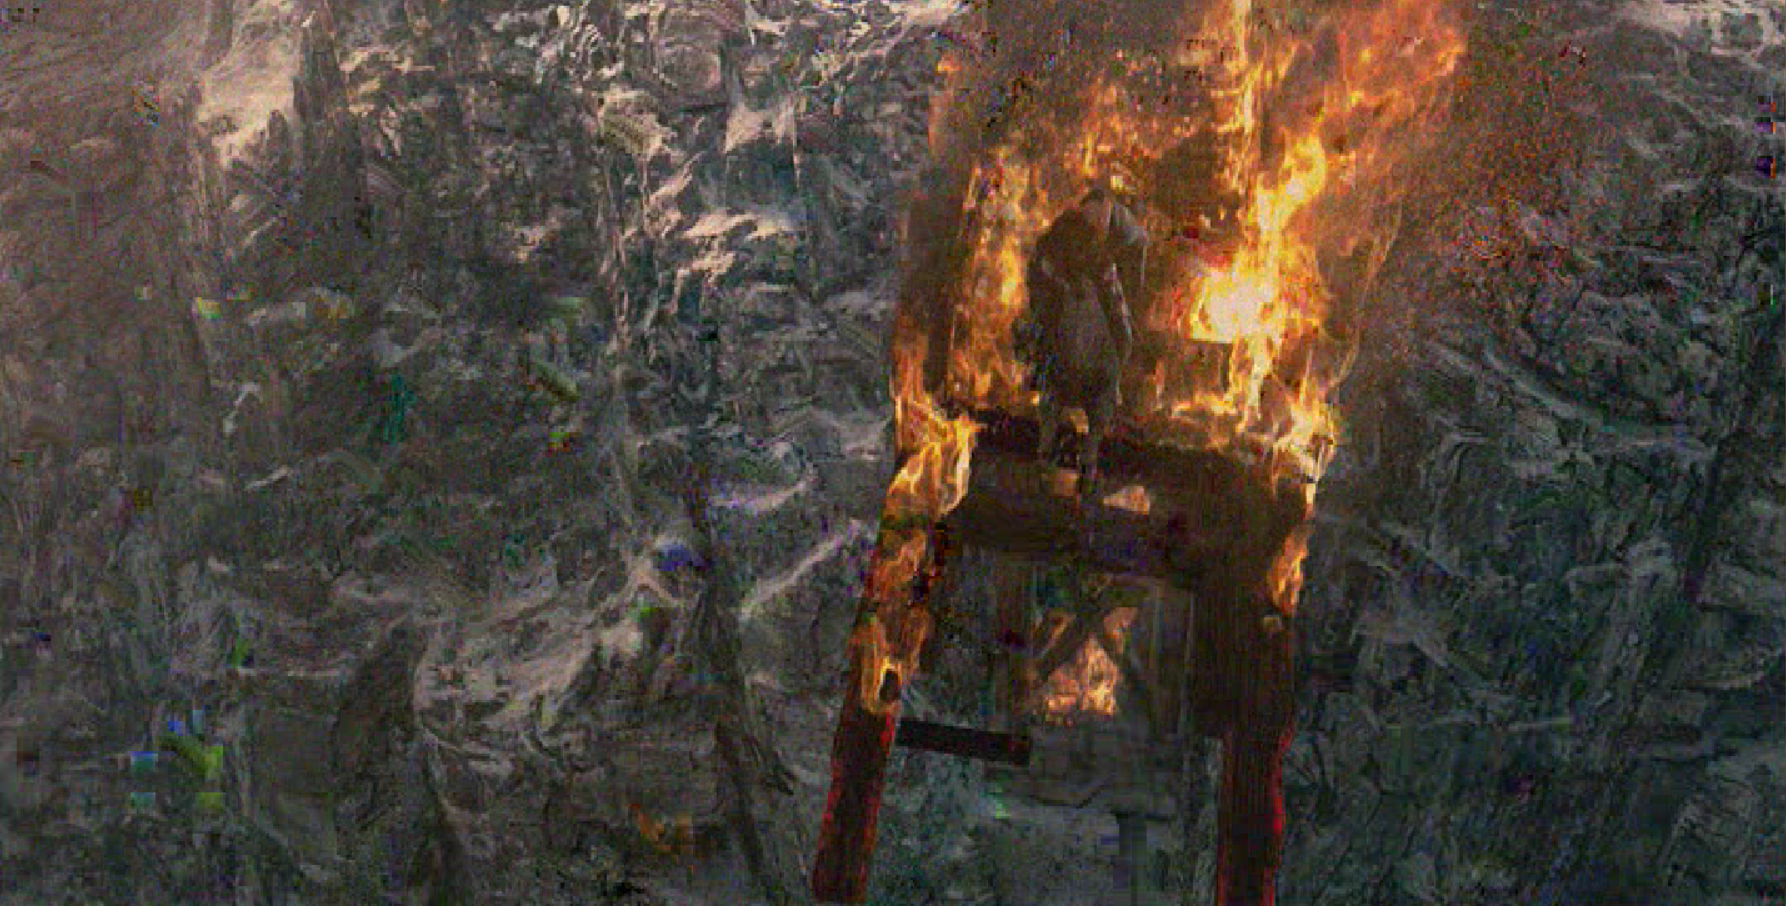
\includegraphics[width=.9\textwidth]{edges}
  \caption{Edge detection}
\end{subfigure}\\
\begin{subfigure}{\textwidth}
  \centering
  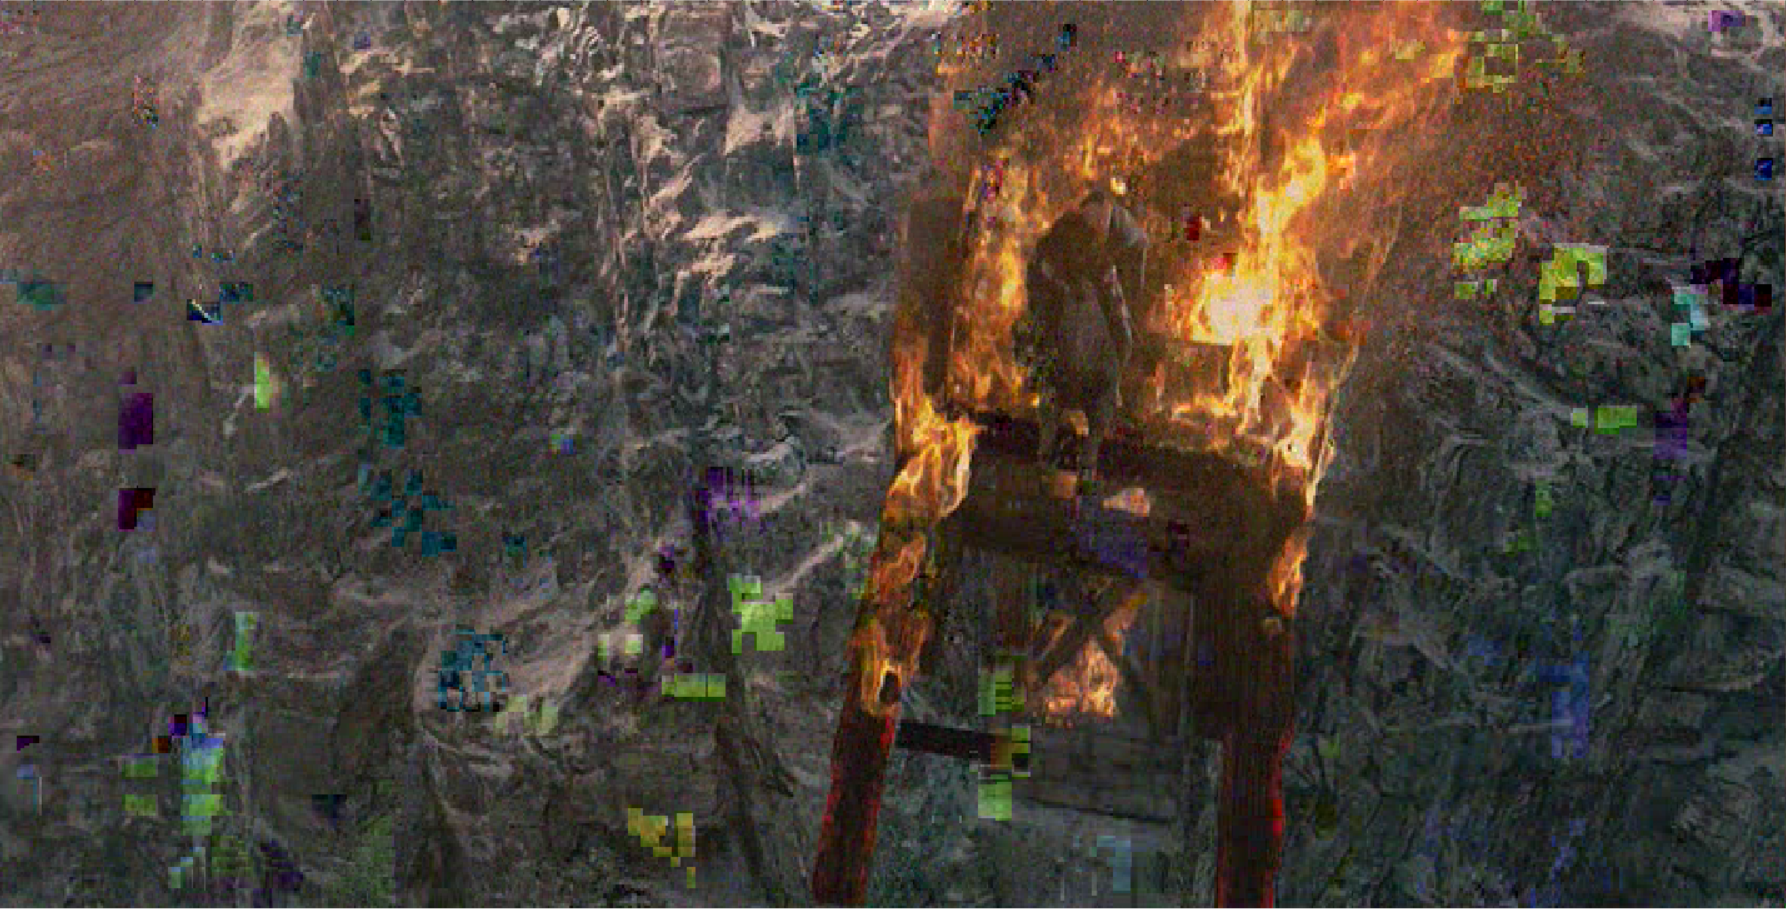
\includegraphics[width=.9\textwidth]{motion}
  \caption{Motion estimation with subblock of size 2}
\end{subfigure}
\caption{The simple pattern is better concealed with the spatial methods than the motion estimation.}
\label{Q7:edgemotion}
\end{figure}

\clearpage

\subsection{Edges compated to motion estimation - complex}
\begin{figure}[ht]
\centering
\begin{subfigure}{\textwidth}
  \centering
  
\includegraphics[width=.9\textwidth]{edgescomplex}
  \caption{Edge detection}
\end{subfigure}\\
\begin{subfigure}{\textwidth}
  \centering
  
\includegraphics[width=.9\textwidth]{motioncomplex}
  \caption{Motion estimation with subblock of size 2}
\end{subfigure}
\caption{The complex pattern is better concealed with the motion estimation.}
\label{Q7:edgemotioncomplex}
\end{figure}

\newpage

\section{Q9}\label{app:Q9}
\begin{figure}[!h]\label{fig:PSNR_simple_pattern}
  \centering
  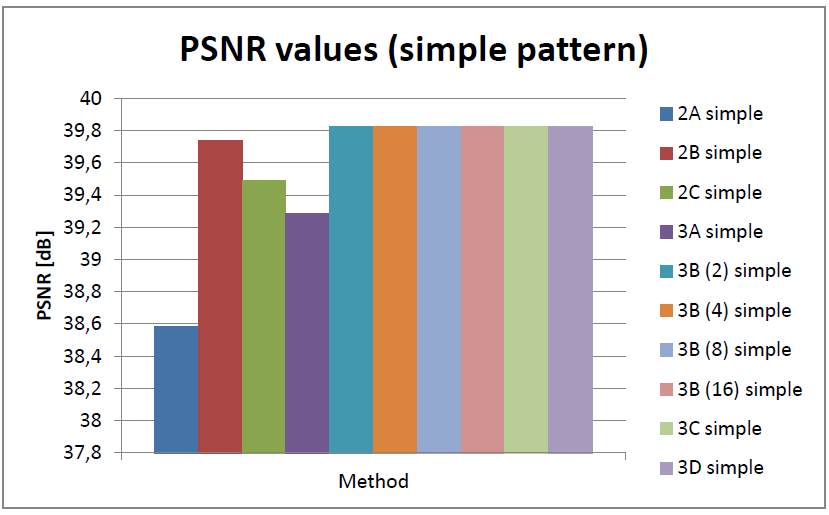
\includegraphics[width=.9\textwidth]{PSNR_simple}
  \caption{Comparison of PSNR values of all methods with the simple error pattern.} 
\end{figure}
\begin{figure}[!h]\label{fig:PSNR_complex_pattern}
  \centering
  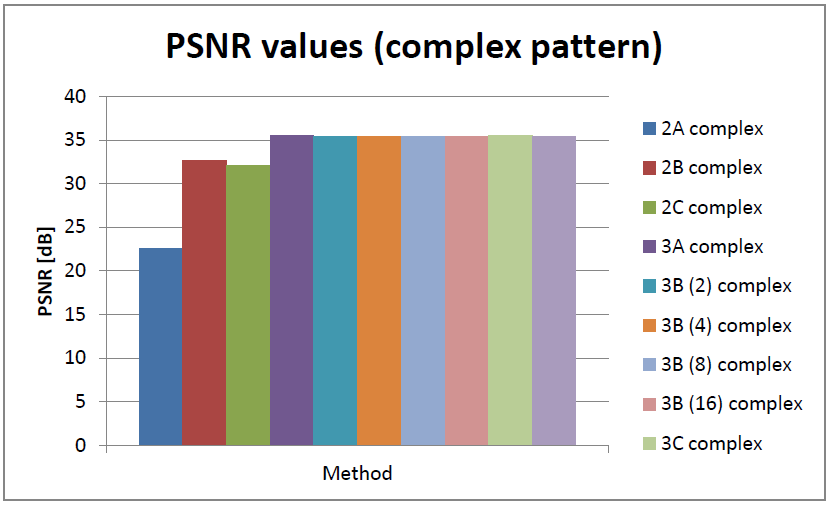
\includegraphics[width=.9\textwidth]{PSNR_complex}
  \caption{Comparison of PSNR values of all methods with the complex error pattern.} 
\end{figure}

\newpage

\section{Q10}\label{app:Q10}
\begin{figure}[!h]\label{fig:SSIM_simple_pattern}
  \centering
  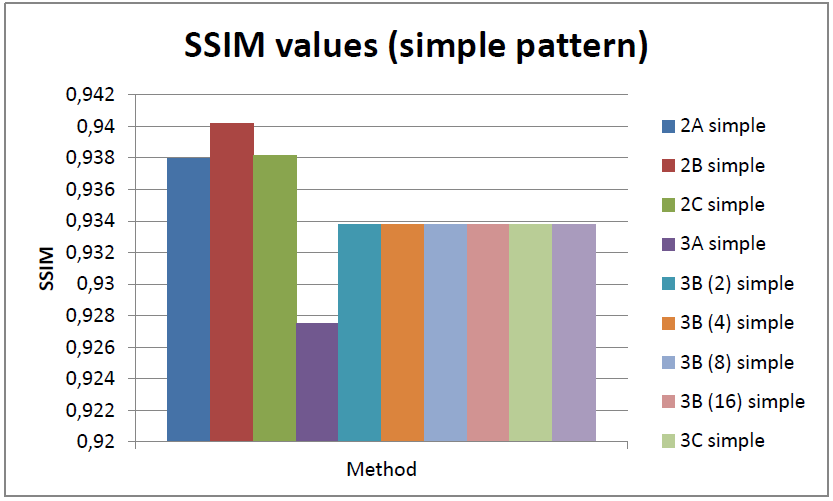
\includegraphics[width=.9\textwidth]{SSIM_simple}
  \caption{Comparison of SSIM values of all methods with the simple error pattern.} 
\end{figure}

\begin{figure}[!h]\label{fig:SSIM_complex_pattern}
  \centering
  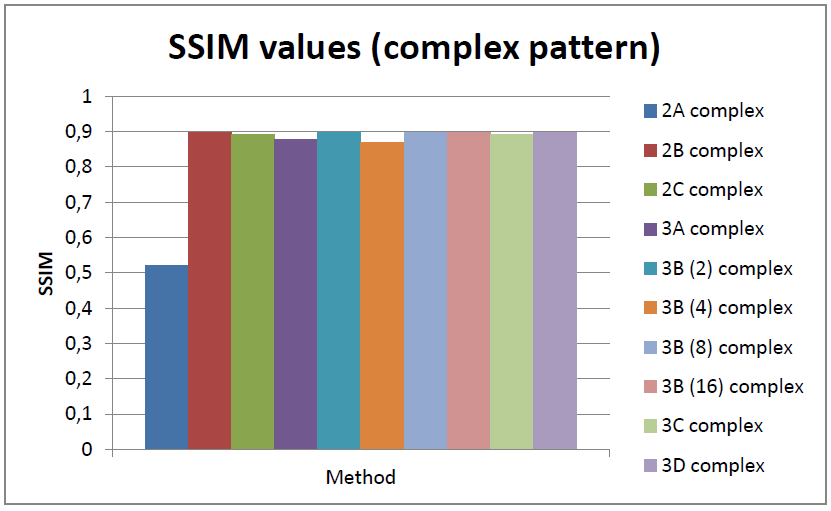
\includegraphics[width=.9\textwidth]{SSIM_complex}
  \caption{Comparison of SSIM values of all methods with the complex error pattern.} 
\end{figure}

\end{appendices}


\end{document}